\documentclass[a4paper,11pt]{article}
\usepackage[latin1]{inputenc}
%\usepackage[T1]{fontenc}
\usepackage[ngerman]{babel}
\usepackage{graphicx}
\usepackage[widemargins]{a4}
\usepackage{amsmath}
\pagestyle{plain}
\parindent0em
\parskip1.5ex plus0.5ex minus0.5ex

\topmargin4mm
\headheight5mm
\headsep6mm
\topskip5mm
\textwidth170mm
\evensidemargin40mm
\oddsidemargin5mm
\textheight220mm
\hoffset -10mm
\footskip10mm
\renewcommand{\textfraction}{0}

%\usepackage{svnkw}
%\svnidlong
%{$HeadURL: $}
%{$LastChangedDate: 2009-08-16 19:09:09 +0200 (Sun, 16 Aug 2009) $}
%{$LastChangedRevision: 529 $}
%{$LastChangedBy: goebl $}
%svnid{$Id: C3_Einfuehrung_Realzeitdatenbasis.tex 529 2009-08-16 17:09:09Z goebl $}


\title{\Large\vspace{-10ex} KogMo-RTDB: Einfuehrung in die Realzeitdatenbasis
              fuer Kognitive Automobile (C3)}
\author{Matthias Goebl (RCS) $<$matthias.goebl*kogmo-rtdb.de$>$ \\ \copyright 2006,2007 Lehrstuhl f�r Realzeit-Computersysteme,  Technische Universit�t M�nchen}
\date{Version 529+}
%\date{Version \svnrev\footnote{Versionskontrolle: Version \svnrev\ vom \svndate, zuletzt geaendert von \svnauthor}\\
%Nur fuer den internen Gebrauch im SFB/TR 28 Kognitive Automobile}
%\date{\today\footnote{Version:
% \$LastChangedRevision: 529 $ - 
%  $LastChangedDate: 2009-08-16 19:09:09 +0200 (Sun, 16 Aug 2009) $ -
%  $LastChangedBy: goebl $ $ \$
%}}
\begin{document}
\selectlanguage{ngerman}

\maketitle
%\tableofcontents

\section{Einfuehrung und Anwendungsbereich}

Ein Kognitives Automobil kann sich in seiner Umgebung nur sicher bewegen,
wenn von der sensoriellen Wahrnehmung (Video, Radar, Lidar) bis zur
Regelung des Fahrzeugs eine schritthaltende Datenverarbeitung garantiert wird.
Dazu muessen zum einen schnelle und deterministische Algorithmen effizient
implementiert werder. Auf der anderen Seite muss eine Laufzeitumgebung
existieren, die diesen Algorithmen die notwendigen Ressourcen wie
Rechenzeit und Speicher zur Verfuegung stellt.

Im SFB/TR 28 "`Kognitive Automobile"' ist es
Aufgabe des Teilprojekts C3, eine realzeitfaehige Entwicklungsplattform
fuer alle Wahrnehmungs-, Kommunikations-, Kooperations- und Verhaltens-Funktionen
zu definieren und bereitzustellen.
Die Definition der zu verwendenden Hardware ist Teil eines weitern Dokuments.
Die hier vorgestellte Realzeitdatenbasis ist Teil der Software dieser Plattform
und dient dem transparenten Datenaustausch zwischen den Software-Modulen
der jeweiligen Teilprojekte.

Die zu erfuellenden (Zeit-)Anforderungen sind grob skizziert:
%wurden wie folgt abgeschaetzt:
\begin{itemize}
\item Zu erwartende Fahrzeuggeschwindigkeit: mindestens $100 \frac{km}{h}$,
      damit bewegt sich das Fahrzeug in der Sekunde mindestens $27.8 m$.
\item Zu erwartende Zykluszeit fuer Sensordaten: maximal $33.3 ms$ bei
      einer angenommenen Videoframerate von $30 \frac{frames}{s}$
\item Das Fahrzeug bewegt sich daher pro angenommenem Zyklus $1 m$ fort
\item Pro Zyklus sollen mindestens 100 Objekte abgefragt und aktualisiert
      werden koennen
\item Die Datenbasis selbst soll dabei auf keinen Fall mehr als 10\% der
      Rechenzeit beanspruchen, da ja die Hauptaufgabe des Systems die
      Wahrnehmung ist
\item Die Datenbasis soll realzeitfaehig sein, d.h. die Antwortzeiten muessen
      kurz und deterministisch sein. Dies impliziert, dass zum Beispiel bei
      einem Speichern nicht erst Daten aufwendig konvertiert, serialisiert oder
      geparst werden duerfen.
\item Im Kognitiven Automobil wird es Wahrnehmungsprozesse mit
      unterschiedlicher zeitlicher Aufloesung geben. Die Datenbasis muss daher
      die verwalteten Daten fuer eine kurze Zeit zwischenspeichern um eine
      zeitliche Entkopplung der Prozesse zu ermoeglichen.
\item Auf die Datenbasis soll programmiersprachenunabhaengig
      zugegriffen werden koennen, z.B. von C, C++, Ada, Java.
\end{itemize}



\section{Funktionalitaet}

%\begin{figure}[htb!]
% \centerline{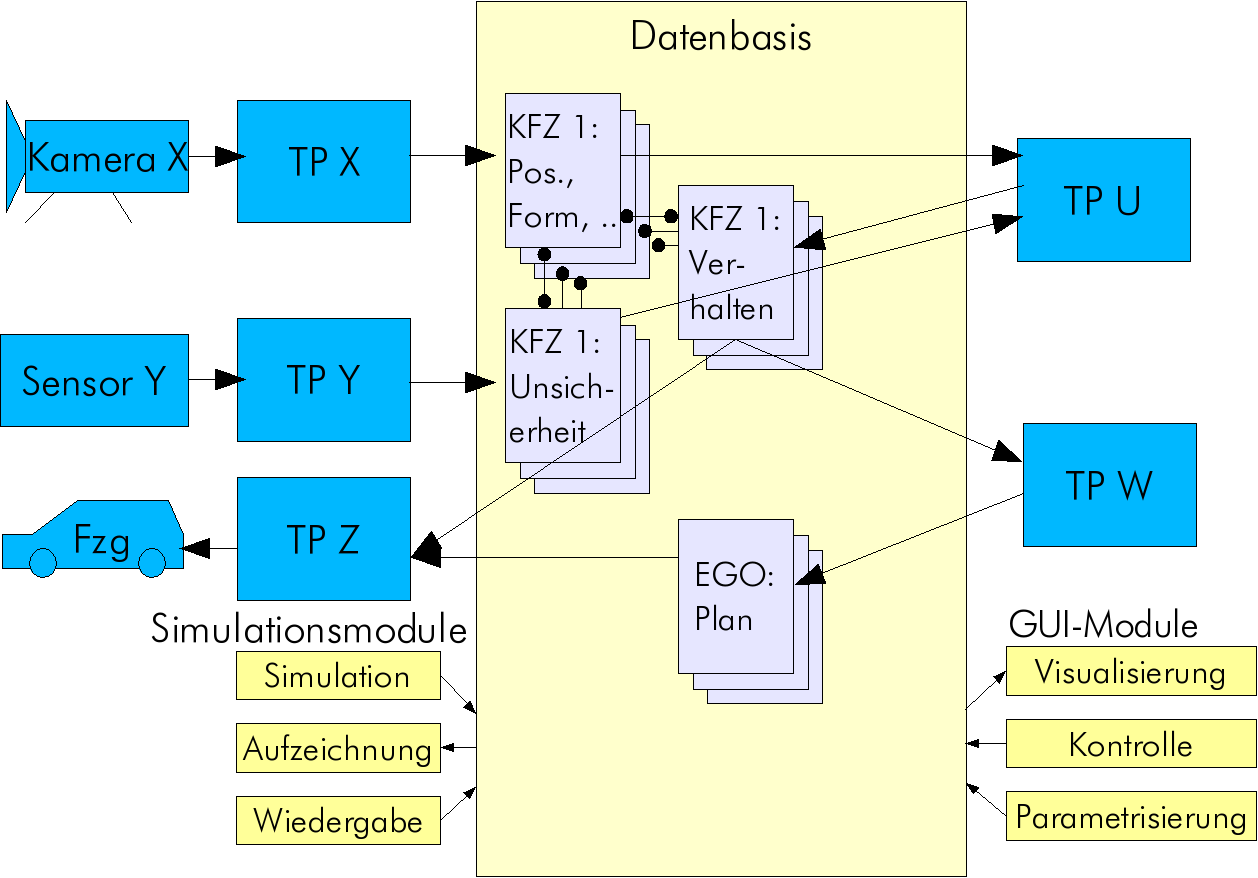
\includegraphics[width=0.7\textwidth]{C3_Einfuehrung_Realzeitdatenbasis_Datenbasis}}
%% \caption{\label{fig:}}
%\end{figure}

Die Realzeitdatenbasis dient als Framework fuer Kommunikation verschiedener TPs:
Jedes Projekt kann Daten publizieren und alle koennen die Daten dann abrufen
(kann man verhindern, wenn man nicht will).
Der Datenbestand wird fuer eine kurze Zeit (z.B. 10 s) in einem Ringpuffer
vorgehalten (die Verwaltung des Ringpuffers geschieht automatisch).
Zur zeitlichen Entkopplung muss bei Abfragen der gewuenschte Zeitpunkt
angegeben werden.
Die zu verwaltenden Daten werden in Datenbloecke gepackt, die hier Objekte
genannt werden. Dies ist aber nicht mit der objektorientierten Programmierung
zu verwechseln - es existiert jedoch auch ein objektorientiertes Interface
fuer die Datenbasis (s.u.).

Grundlegende Funktionen der Datenbasis:
\begin{itemize}
\item Neues Objekt, bestehend aus Informationsblock (Name, Besitzer, ...)
      und Datenblock (beliebiger Inhalt) anlegen und wieder loeschen
\item Datenblock eines Objekt aktualisieren
\item Nach Object mit bestimmten Attributen im Informationsblock
      suchen, sowie Informations- und Datenblock abrufen
\item Datenblock zu einem bestimmten Zeitpunkt abrufen, sofern verfuegbar
\item Auf die Aktualisierung eines Datenblocks warten ("`Trigger"')
\item Auf das Anlegen eines bestimmten Objekts warten
\end{itemize}

Die Spezifikation der genauen Inhalte ist nicht Aufgabe von C3, dies geschieht
in der QAG3. In der SAG2 wurde durch die Spezifikation von CSV-Dateien
zum Datenaustausch fuer die Simulation eine sehr gute Arbeitsgrundlage gelegt.
Aus den im Kopf der CSVs enthaltenen Parametern fuer einen Simulationsschritt
laesst sich ein Datenblock definieren.
Darueber lassen sich dann auch simulierte Daten einspielen.

%QAG3/SAG2: Benoetigt werden noch weitere gemeinsame Bezeichnungen, Modelle, Begriffe,
%Koordinatensysteme, Wissensformulierung, uvm..

%\begin{figure}[htb!]
% \centerline{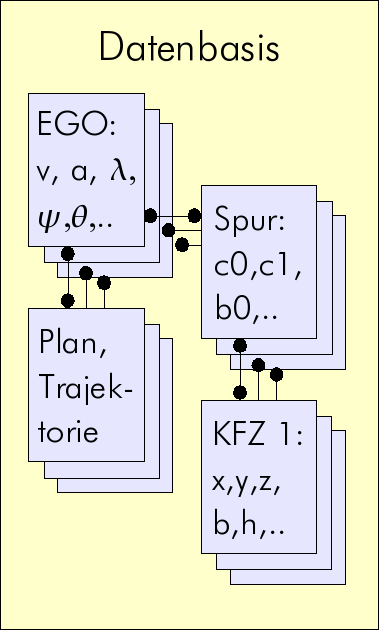
\includegraphics[width=0.2\textwidth]{C3_Einfuehrung_Realzeitdatenbasis_Objekte}}
% \caption{\label{fig:}}
%\end{figure}


\clearpage
\section{Struktur der Daten}

Jedes "`Objekt"' in der Datenbasis besteht aus einem Informationsblock, der beim
Eintragen des Objekts einmalig angelegt wird, und einem Datenblock, der sich periodisch aendert.

\subsection{Der Informationsblock (Datencontainer/Metadata)}
Der Informationsblock enthaelt die Metadaten eines Objekts,
er ist wie ein "`Etikett"'. Er laesst sich voraussichtlich nach
dem Anlegen eines Objekts nicht mehr aendern\footnote{Problem: was tun, wenn sich der 
Typ eines Objekts aendert? Moegliche Alternative: Ein neues Objekt "`ersetzt"' ein altes,
d.h. es wird "`atomar"' geloescht und neu angelegt, ausserdem wird ein Link von dem geloeschten
auf das neue gesetzt}. Er enthaelt folgende Daten:

\begin{tabular}{|l|l|l|}
\hline\multicolumn{3}{|c|}{\bf Inhalte des statischen Informationsblocks eines jeden Realzeit-Datenbasis-Objekts} \\ \hline
Datenfeldname			& Datentyp				& Beschreibung \\ \hline
\hline\multicolumn{3}{|c|}{Vom Benutzer vorzugebende Daten} \\ \hline
\small\verb!otype!		& \small\verb!kogmo_rtdb_objtype_t!	& Objekt-Typkennung \\ \hline
\small\verb!name!		& \small\verb!kogmo_rtdb_objname_t!	& Beliebiger Name, beginnend mit Teilprojekt, z.B. c3\_test \\ \hline
\small\verb!parent_oid!		& \small\verb!kogmo_rtdb_objid_t!	& Objekt-ID des Vaterobjekts in einem hierarchischen \\
				&					& Szenenbaum. 0=unverlinkt \\ \hline
\small\verb!size_max!		& \small\verb!kogmo_rtdb_objsize_t!	& Maximale Groesse, die ein Datencontainer annehmen kann \\ \hline
\small\verb!history_interval!	& \small\verb!float!			& Zeitspanne, fuer die alte Versionen von geaenderten \\
				&					& Datencontainern in einem Ringpuffer aufgehoben werden \\ \hline
\small\verb!avg_cycletime!	& \small\verb!float!			& Angenommene Zykluszeit fuer Aktualisierungen des \\
				&					& Datencontainers \\ \hline
\small\verb!max_cycletime!	& \small\verb!float!			& Maximale Zykluszeit \\ \hline
\small\verb!flags.read_deny!	& \small\verb!bool!			& 1= andere Prozesse duerfen den Datencontainer nicht lesen \\
				&					& 0= jeder darf lesen (default) \\ \hline
\small\small\verb!flags.write_allow!& \small\verb!bool!			& 1= andere Prozesse duerfen den Datencontainer aktualisieren\\
				&					& 0= nur der Besitzer nur aktualisieren (default) \\ \hline
\small\verb!flags.unique!	& \small\verb!bool!			& 1= Einzigartiger Objekttyp, d.h. es duerfen keine anderen \\
				&					& ~~~~~Objekte dieses Typs existieren \\
				&					& 0= beliebig viele Objekte dieses Typs (default) \\ \hline
\hline \multicolumn{3}{|c|}{Von der RTDB automatisch eingesetzte Daten} \\ \hline
\small\verb!oid!		& \small\verb!kogmo_rtdb_objid_t!	& Eindeutige Objekt-ID \\ \hline
\small\verb!created_ts!		& \small\verb!kogmo_timestamp_t!	& Zeitpunkt, zu dem das Objekt in die RTDB eingetragen \\
				&					& wurde \\ \hline
\small\verb!created_proc!	& \small\verb!kogmo_rtdb_objid_t!	& Objekt-ID des Prozesses, der das Objekt in die RTDB \\
				&					& eingetragen hat \\ \hline
\small\verb!deleted_ts!		& \small\verb!kogmo_timestamp_t!	& 0 (Objekt wurde nicht geloescht) oder Zeitpunkt, zu \\
				&					& dem das Objekt geloescht wurde \\ \hline
\small\verb!deleted_proc!	& \small\verb!kogmo_rtdb_objid_t!	& 0 oder Objekt-ID des Prozesses, der das Objekt geloescht hat \\ \hline
\end{tabular}

Die obigen Datentypen sind in \verb!kogmo_rtdb_types.h! definiert, der Informationsblock ist
ein \\ \verb!kogmo_rtdb_obj_info_t! (typedef struct).

\subsubsection{Suche nach Objekten}
Eine Suche nach Objekten in der Datenbasis (mittels \verb!kogmo_rtdb_obj_searchinfo()!)
kann nach folgenden Kriterien geschehen:
\begin{itemize}
\item Name (mit der Moeglichkeit von regular Expressions)
\item Objekt-ID
\item Objekt-Typ
\item Objekt-ID des Vaters
\item Objekt-ID des Prozesses, der das Objekt eingefuegt hat
\item Zeitpunkt, zu dem das Objekt existiert(e)
\end{itemize}


\subsection{Der Datenblock eines Objekts (Dateninhalte)}

Der Datenblock eine Objekts ist der Teil des Objekts, der sich periodisch,
z.B. mit dem Videozyklus von 33ms, aendert. Die vergangenen Inhalte
des Datenblocks werden ueber eine vorher spezifizierte Zeit (history\_interval)
in Ringpuffern gelagert, bevor sie ueberschrieben werden.
Damit ist es moeglich, dass auch Wahrnehmungsprozesse mit einer niedrigeren Periode, z.B. 0,5~Sekunden,
die angefallenen Daten auswerten, ohne dabei Daten zu verliegen oder Inkonsistenzen
zu bekommen\footnote{Die Laufzeit der Wahrnehmungsprozesse darf dabei natuerlich
nicht laenger als die spezifizierte Zeit history\_interval sein}.

Um die zeitliche konsistenz bei mehreren Abfragen innerhalb eines Zyklus
zu bewahren, ist es sinnvoll, sich zu Beginn des Zyklus einen
Zeitstempel zu holen, und diesen fuer alle Abfragen innerhalb dieses Zyklus
zu verwenden. Die RTDB liefert dann jeweils die Daten, die fuer den
gegebenen Zeitpunkt gueltig waren. Diese schliesst auch die Daten von
geloeschten Objekten ein: diese bleiben auch nach dem Loeschen fuer
mindestens die Zeit history\_interval in der RTDB!

Der Datenblock kann fast beliebige Daten enthalten, er muss jedoch
mit folgender Struktur beginnen:

\begin{tabular}{|l|l|l|}
\hline\multicolumn{3}{|c|}{\bf Basis-Inhalte des dynamischen Datenblocks eines jeden Realzeit-Datenbasis-Objekts} \\ \hline
Datenfeldname			& Datentyp				& Beschreibung \\ \hline
\hline\multicolumn{3}{|c|}{Vom Benutzer vorzugebende Daten} \\ \hline
\small\verb!size!		& \small\verb!kogmo_rtdb_objsize_t!	& Objektgroesse, mindestens die Groesse dieses Basisblocks \\
				&					& maximal \small\verb!size_max! aus dem Informationsblock \\ \hline
\small\verb!data_ts!		& \small\verb!kogmo_timestamp_t!	& Zeitpunkt, auf den sich die Daten beziehen, bei einem \\
				&					& Videobild z.B. die Zeit der Aufname \\ \hline
\hline \multicolumn{3}{|c|}{Von der RTDB automatisch eingesetzte Daten} \\ \hline
\small\verb!committed_ts!	& \small\verb!kogmo_timestamp_t!	& Zeitpunkt, zu dem diese Daten in die RTDB \\
				&					& eingetragen wurden \\ \hline
\small\verb!committed_proc!	& \small\verb!kogmo_rtdb_objid_t!	& Objekt-ID des Prozesses, der diese Daten in die RTDB \\
				&					& eingetragen hat \\ \hline
\end{tabular}


\subsection{Eigene Datenbloecke, von Teilprojekten definiert}

Die einzelnen Teilprojekte koennen sich eigene Objekte definieren, die sich in der
Definition der Inhalte der Datenbloecke unterscheiden. Voraussetzung ist, dass
ein Datenblock mit obigem Basis-Datenblock beginnt.
Praktisch sieht das so aus:
\begin{verbatim}
typedef struct {
  kogmo_rtdb_subobj_base_t      base;   // Basisdaten, siehe oben
  kogmo_rtdb_subobj_TP_XXXXXX_t XXXXXX; // Eigener Datenblock XXXXXX des Teilprojekts TP
} kogmo_rtdb_obj_TP_XXXXXX_t;           // Gesamt-Datenblock eines solchen Objekts
\end{verbatim}

Wie man ein den Datenblock fuer ein eigenes Objekt definiert zeigt Kapitel~\ref{erweiterung}

\subsubsection{Suche nach Objektinhalten}

Hier ist verfuegbar:
\begin{itemize}
\item Suche nach Daten, die zu einem gegeben Zeitpunkt zuletzt geschrieben wurden (d.h. nach commited\_ts)
\item Suche nach Daten, deren Datenzeitstempel juenger als ein gegebener ist
\item Suche nach Daten, deren Datenzeitstempel aelter als ein gegebener ist
\end{itemize}




\clearpage
\section{Uebersicht ueber das API der Datenbasis}

Alle (C-)Funktionen liefern im Fehlerfall einen negativen Wert.
\\
Die C++-Klassen werfen einen DBError.

\subsection{Verbindung auf- und abbauen}

Die Informationen ueber die beabsichtigte Verbindung werden erst
in ein\\
\verb!kogmo_rtdb_connect_info_t dbinfo! eingetragen:\\
\verb!kogmo_rtdb_connect_initinfo (&dbinfo, "", "a2_roadtracker_example", 0.033)!\\
a2\_roadtracker\_example ist der beabsichtigte eigene Prozessname, 0.033 die
geschaetzte Prozesszykluszeit (wird spaeter verwendet, um tote Prozesse zu
finden.

\verb!kogmo_rtdb_connect (&dbc, &dbinfo)! baut nun die Verbindung auf und
traegt den eigenen Prozess ein. Das Handle \verb!kogmo_rtdb_handle_t *dbc!
wird nun fuer alle weiteren Anfragen benutzt (dann ohne \&).

Den Verbindungsabbau erledigt \verb!kogmo_rtdb_disconnect(dbc, NULL)!.


In C++ geschieht der Verbindungsaufbau so, ein Abbau ist nicht noetig:\\
\verb!RTDBConn DBC("a2_roadtracker_example_cxx", 0.033, "")!


\subsection{Objekte hinzufuegen, suchen und loeschen}

Durch das Einfuegen eines Objekte wird ein "`Datencontainer"' mit einem "`Etikett"'
erstellt. Das Etikett enthaelt die (z.Zt. noch) unveraenderlichen Metadaten
eines Objekts, wie ID, Name, Typ, Maximal-Containergrosse, Erstellungszeit
und Besitzerprozess.

Die Datencontainer werden dann z.B. mit \verb!kogmo_rtdb_obj_writedata()! (s.u.)
beschrieben. Dabei wird eine Kurzzeit-Historie mit den letzten Veraenderungen
in einem Ringpuffer gehalten. Die dabei notwendigen Locking-Mechanismen
sind Teil der Datenbasis.

\begin{itemize}
\item \verb!kogmo_rtdb_obj_info_t!: Struct, das Object-Metadaten enthaelt (Etikett)
\item \verb!kogmo_rtdb_obj_initinfo()!: Objekt-Metadaten initialisieren (Etikett saubermachen)
\item \verb!kogmo_rtdb_obj_insert()!: Objekt anlegen (Erstellt neues Objekt mit den
Daten des Etiketts, legt Datencontainer fuer zukuenftige Inhalte an)
\item \verb!kogmo_rtdb_obj_delete()!: Objekt loeschen (Loescht das Objekt, dessen
 Etikett, und alle Datencontainer). Aber nicht sofort: je nach History-Tiefe
 bleiben die Inhalte noch ein paar Sekunden in der Datenbasis und koennen
 mit einem Zeitstempel der Vergangenheit noch referenziert werden.
 Damit kann man langsamen Warnehmungsprozessen nicht die Daten unter
 dem Hintern wegziehen.
\item \verb!kogmo_rtdb_obj_readinfo()!: Objekt-Metadaten zu einer ID holen
\item \verb!kogmo_rtdb_obj_searchinfo()!: Objekte mit bestimmten Metadaten (UND-Verknuepfung)
suchen und ersten Treffer oder als Liste von IDs zurueckgeben.
\item \verb!kogmo_rtdb_obj_searchinfo_wait()!: Objekt(e) suchen. Wenn nicht vorhanden,
warten, bis ein anderer Prozess ein solches Objekt anlegt.
\item \verb!kogmo_rtdb_obj_dumpinfo_str()!: Objekt-Metadaten in einen String packen.
\end{itemize}


\subsection{Objektinhalte schreiben, lesen und durchsuchen}
Wenn man nun einen Container angelegt oder gefunden hat, hat man nun eine
eindeutige Objekt-ID~(OID), die dieses referenziert.

\begin{itemize}
\item \verb!kogmo_rtdb_obj_initdata()!: Damit wird ein lokaler Container initialisiert, den man dann beschreiben kann.
\item \verb!kogmo_rtdb_obj_writedata()!: Damit wird der Inhalt des lokalen Containers in die Datenbank kopiert.
\item \verb!kogmo_rtdb_obj_readdata()!: Damit wird der Inhalt eines Containers aus der Datenbank in den lokalen Containers kopiert.
\end{itemize}

Jeder Objektcontainer hat 2 Zeitstempel: Einen Commit-Timestamp, der eher die Datenbank interessiert,
und einen Data-Timestamp, der den Zeitpunkt der Datenentstehung haben sollte, bei einem Bild z.B.
der Aufnahmezeitpunkt. Der Commit-Timestamp wird automatisch beim Schreiben von Daten eingefuegt,
um den Data-Timestamp muss sich die Applikation selbst kuemmern: Wenn die Bilddaten verarbeitet sind,
sollte das Ergebnis ebenfalls den Aufnahmezeitpunkt als Data-Timestamp haben. An der Differenz der
Commit-Timestamps sieht man, wie lange die Applikationen gerechnet haben.

Da sich der Inhalt der Datenbasis fortwaehrend aendert, ist es wichtig mit konsistenten Daten zu rechnen.
Daher muss man zu jeder Anfrage einen Timestamp mitgeben (bei "`0"' wird fuer Faulpelze die aktuelle Zeit
eingesetzt).

\verb!kogmo_rtdb_obj_readdata()! bezieht sich auf den Commit-Timestamp, d.h. den letzten Datensatz, der
zum gegebenen Zeitpunkt aktuell war.

Achtung: Wenn man auf ein Objekt mit \verb!kogmo_rtdb_obj_searchinfo_wait()! gewartet hat, sollte man
mit \verb!kogmo_rtdb_obj_readdata_waitnext()! das erste mal darauf zugreifen, da sich der Ersteller
des Objekts zwischen dem \verb!kogmo_rtdb_obj_insert()! und dem ersten \verb!kogmo_rtdb_obj_writedata()!
beliebig Zeit lassen kann und es sehr wohl erlaubt ist, dass die Metadaten da sind aber (noch) keine
Daten.


\begin{itemize}
\item \verb!kogmo_rtdb_obj_readdata_older()!: Liefert den Datensatz, dessen Data-Timestamp
weiter in der Vergangenheit liegt als der gegebene.
\item \verb!kogmo_rtdb_obj_readdata_younger()!: Liefert den Datensatz, dessen Data-Timestamp
weiter in der Zukunft liegt als der gegebene.
\item \verb!kogmo_rtdb_obj_readdata_waitnext()!: Wartet darauf, dass ein anderer Prozess den Datensatz
aktualisiert (schreibt) und liefert ihn dann.
\end{itemize}

Die obigen Funktionen kopieren ihre Daten; Funktionen, die auf die Datenbasis direkt, ohne Kopie zugreifen
werden bald freigegeben.



\subsection{Prozesssynchronisation}
\verb!kogmo_rtdb_cycle_done!: Sollte von jedem Prozess am Ende jedes Zyklus aufgerufen werden.
Andere Prozesse koennen dann ein \verb!kogmo_rtdb_obj_readdata_waitnext()! auf das
Prozess-Objekt machen und werden dann aufgeweckt, wenn der Prozess fertig ist.

Alternativ kann man auf die Aenderung eines bestimmten Daten-Objektes warten. Dabei wird
es wichtig, in welcher Reihenfolge der zeitlich fruehere Prozess seine Objekte aktualisiert.
Dies ist Vereinbarungssache zwischen den Teilprojekten, im Laufe des SFBs wird es sich zeigen,
ob ein "`bulk-commit"' ueber mehrere Objekte auf einmal notwendig wird.


\begin{figure}[htb!]
 \centerline{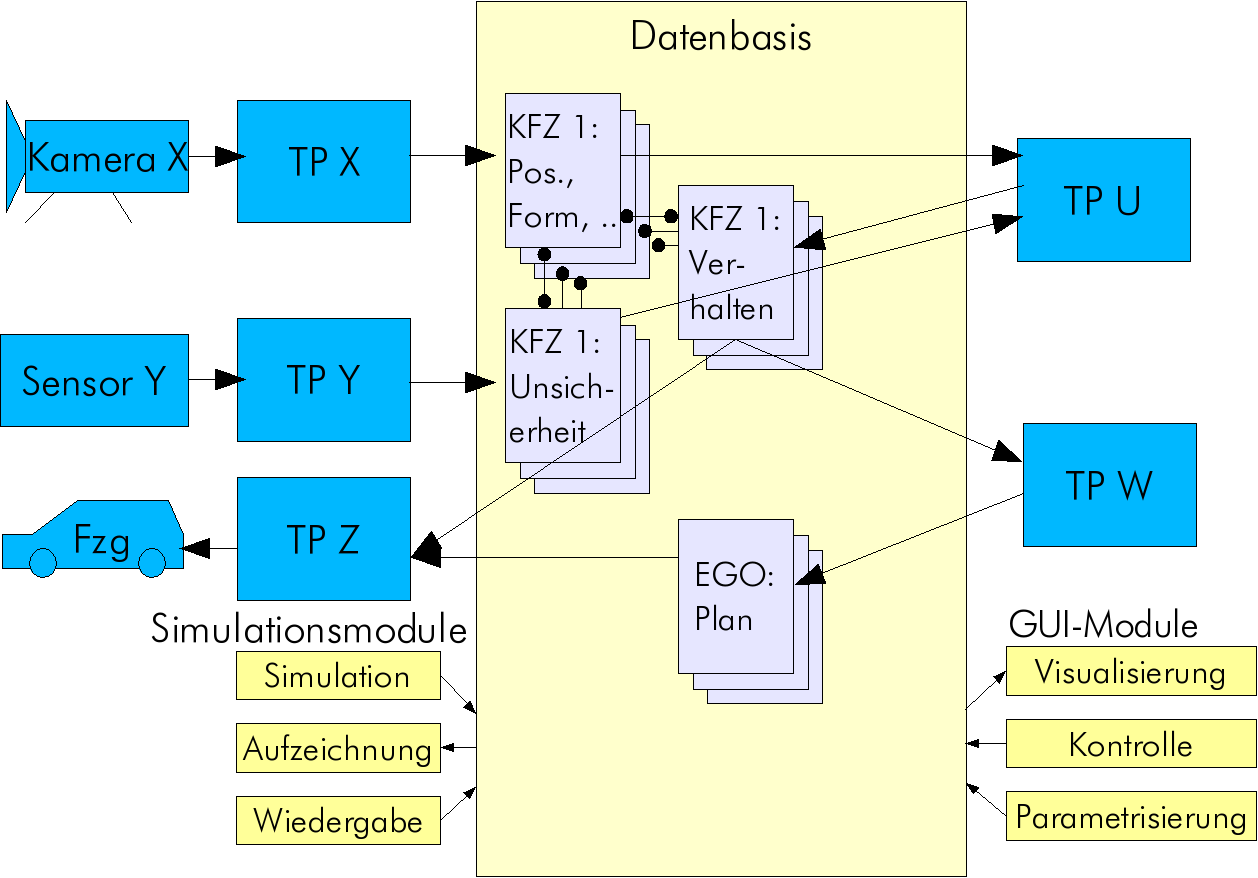
\includegraphics[width=0.7\textwidth]{C3_Einfuehrung_Realzeitdatenbasis_Datenbasis}}
 \caption{\label{fig:schema}Skizze der Datenbasis}
\end{figure}


\clearpage
\section{Erweiterung um ein neues Datenobjekt}
\label{erweiterung}

\begin{enumerate}

\item Die Datei
      \verb! objects/kogmo_rtdb_obj_typeids.h !
      editieren und die Typliste um eigenen Objekttyp ergaenzen und eigene Includes hinzufuegen:
\vspace{-1.5ex}\scriptsize\begin{verbatim}
enum kogmo_rtdb_objtype {
...
  // A2: Spurdaten nach Klothoidenmodell, erste Version:
  KOGMO_RTDB_OBJTYPE_A2_ROADKLOTH_V1 =       0xA20101,
...
};
...
// A2:
#include "kogmo_rtdb_obj_a2.h"     
...
\end{verbatim}\normalsize

\item Wir gehen aus von der CSV-Beschreibung (A2\_fahrspur.csv):\\
\vspace{-1.5ex}\scriptsize\begin{verbatim}
# Spezifikations-Datei A2_Spec_Fahrspur.txt V 0.0 (RCS/TAS)
# Eigenfahrspur als Klothoide modelliert. 
time[ns];n[];l_0[m];c0_0[rad/m];c1_0[rad/m^2];b0_0[m];b1_0[m/m];l_1[m];c0_1[rad/m];c1_1[rad/m^2];b0_1[m];b1_1[m/m];...
1149691630000000000;5;100.0;0.0;0.0;3.80;0.0;100;0.0;1.0e-4;3.80;0.0;100;1.0e-2;0.0;3.80;0.0;25;1.0e-2;-4.0e-4;3.80;...
...
\end{verbatim}\normalsize


\item Die Datei \verb! kogmo_rtdb_obj_a2.h ! erstellen:
\vspace{-1.5ex}\scriptsize\begin{verbatim}
/*! \addtogroup kogmo_rtdb_objects */ /*@{*/
//! Maximalanzahl der Segmente im folgenden Klothoidenmodell
#define A2_ROADKLOTH_SEGMAX 5

/*! \brief Eigenfahrspur als Klothoide modelliert
 * Modellbeschreibung wie folgt/zu finden in: ...
 */
typedef struct
{
 int n;
   //!< Anzahl der Segmente (d.h. wieviele Eintraege der folgenden Arrays
   //!< gueltig sind)
 float l [A2_ROADKLOTH_SEGMAX];
   //!< Segmentlaenge
 float c0 [A2_ROADKLOTH_SEGMAX];
   //!< Kruemmung
 float c1 [A2_ROADKLOTH_SEGMAX];
   //!< Kruemmungsaenderung
 float b0 [A2_ROADKLOTH_SEGMAX];
   //!< Breite
 float b1 [A2_ROADKLOTH_SEGMAX];
   //!< Breitenaenderung
} kogmo_rtdb_subobj_a2_roadkloth_t;

/*! \brief Vollstaendiges Objekt mit Spurdaten
 */
typedef struct
{
  kogmo_rtdb_subobj_base_t base;
    //!< Basisdaten
  kogmo_rtdb_subobj_c3_sixdof_t sixdof;
    //!< Relativpostion zum projizierten Fahrzeug-Schwerpunkt-Koordinatensystem (K_CGP)
  kogmo_rtdb_subobj_a2_roadkloth_t roadkloth;
    //!< Die Daten des eigentlichen Klothoidenmodells
} kogmo_rtdb_obj_a2_roadkloth_t;
\end{verbatim}\normalsize

\item In der Datei \verb! kogmo_rtdb_obj_a2_funcs.h! koennte man Funkionen
      definieren, die (unter C) auf diesen Daten arbeiten. Im einfachsten
      Fall koennte hier eine Funktion definiert sein, die die Daten in eine
      Textform bringt ("`dump"').\\
      Dann muss man \verb! objects/kogmo_rtdb_obj_funcs.h !
      ergaenzen:
\vspace{-1.5ex}\scriptsize\begin{verbatim}
...
// A2:
#include "kogmo_rtdb_obj_a2_funcs.h"
...
\end{verbatim}\normalsize

\item In der Datei \verb!kogmo_rtdb_obj_a2_classes.h! koennte man nun
      Klassen definieren, die diese Daten in eine Klasse packen ("`wrappen"')
      und inline definiert sind (damit bleibt das Interface "`C"'). \\
      Dann muss man \verb! objects/kogmo_rtdb_obj_classes.hxx !
      ergaenzen:
\vspace{-1.5ex}\scriptsize\begin{verbatim}
...
// A2:
#include "kogmo_rtdb_obj_a2_classes.hxx"
...
\end{verbatim}\normalsize

%\item Obige Dateien ins Subversion committen und neue Dateien hinzufuegen:\\
%      \verb! $ svn add kogmo_rtdb_obj_a2{.h,_funcs.h,_classes.hxx} ! \\
%      \verb! $ svn diff | less  # Aenderungen ueberpruefen ! \\
%      \verb! $ svn commit !

\end{enumerate}







\clearpage
\section{Beispiel: Ein Objekt anlegen und periodisch aktualisieren}

\scriptsize
%../examples/kogmo_rtdb_writer.c
\begin{verbatim}
#include <stdio.h> /* printf */
#include <unistd.h> /* sleep,getpid */
#include <math.h> /* sin,cos */
#include "kogmo_rtdb.h"

#define DIEonERR(value) if (value<0) { \
 fprintf(stderr,"%i DIED in %s line %i with error %i\n",getpid(),__FILE__,__LINE__,-value);exit(1);}

int
main (int argc, char **argv)
{
  kogmo_rtdb_handle_t *dbc;
  kogmo_rtdb_connect_info_t dbinfo;
  kogmo_rtdb_obj_info_t roadobj_info;
  kogmo_rtdb_obj_a2_roadkloth_t roadobj;
  kogmo_rtdb_objid_t oid;
  int err, i, imax;
  
  // Verbindung zur Datenbasis aufbauen, unsere Zykluszeit is 33 ms
  err = kogmo_rtdb_connect_initinfo (&dbinfo, "", "a2_roadtracker_example", 0.033); DIEonERR(err);
  oid = kogmo_rtdb_connect (&dbc, &dbinfo); DIEonERR(oid);

  // Object fuer Fahrspur erstellen
  err = kogmo_rtdb_obj_initinfo (dbc, &roadobj_info,
    "a2_eigenfahrspur", KOGMO_RTDB_OBJTYPE_A2_ROADKLOTH_V1, sizeof (roadobj)); DIEonERR(err);
  oid = kogmo_rtdb_obj_insert (dbc, &roadobj_info); DIEonERR(oid);

  // Datenobjekt initialisieren
  err = kogmo_rtdb_obj_initdata (dbc, &roadobj_info, &roadobj); DIEonERR(err);

  // Fixe Werte eintragen
  roadobj.sixdof.x     = 2.5;
  roadobj.sixdof.y     = 0;
  roadobj.sixdof.z     = -0.5;
  roadobj.sixdof.yaw   = 0;
  roadobj.sixdof.pitch = 0;
  roadobj.sixdof.roll  = 0;

  imax = 100; // demo
  for ( i=1; i<=imax; i++ )
    {
      // Von welchem Zeitpunkt sind die Daten?
      roadobj.base.data_ts = kogmo_timestamp_now();
      // Nun die eigentlichen Daten (Achtung: sinnlos! Nur zur Demo!)
      roadobj.roadkloth.n=1; // nur ein Klothoidensegment
      roadobj.roadkloth.l[0] = 1.5; // Beispieldaten, die sich aendern...
      roadobj.roadkloth.c0[0] = 10.0*i;
      roadobj.roadkloth.c1[0] = 10.0/i;
      roadobj.roadkloth.b0[0] = sin((float)i/imax);
      roadobj.roadkloth.b1[0] = cos((float)i/imax);

      // Daten schreiben
      err = kogmo_rtdb_obj_writedata (dbc, roadobj_info.oid, &roadobj); DIEonERR(err);

      sleep (1); // Zykluszeit 1s zur Demo
    }

  err = kogmo_rtdb_obj_delete (dbc, &roadobj_info); DIEonERR(err);
  err = kogmo_rtdb_disconnect (dbc, NULL); DIEonERR(err);
  return 0;
}
\end{verbatim}
\normalsize




\clearpage
\section{Beispiel: Ein Objekt finden und dessen Aenderungen verfolgen}

\scriptsize
%../examples/kogmo_rtdb_reader.c
\begin{verbatim}
/*! \file kogmo_rtdb_reader.c
 * \brief Example for reading from the RTDB
 *
 * Copyright (c) 2005,2006 Matthias Goebl <matthias.goebl*goebl.net>
 *     Lehrstuhl fuer Realzeit-Computersysteme (RCS)
 *     Technische Universitaet Muenchen (TUM)
 */

#include <stdio.h> /* printf */
#include <unistd.h> /* getpid */
#include "kogmo_rtdb.h"

#define DIEonERR(value) if (value<0) { \
 fprintf(stderr,"%i DIED in %s line %i with error %i\n",getpid(),__FILE__,__LINE__,-value);exit(1);}

int
main (int argc, char **argv)
{
  kogmo_rtdb_handle_t *dbc;
  kogmo_rtdb_connect_info_t dbinfo;
  kogmo_rtdb_obj_info_t roadobj_info;
  kogmo_rtdb_obj_a2_roadkloth_t roadobj;
  kogmo_rtdb_objid_t oid;
  int err;
  
  // Verbindung zur Datenbasis aufbauen, unsere Zykluszeit is 33 ms
  err = kogmo_rtdb_connect_initinfo (&dbinfo, "", "a2_roadviewer_example", 0.033); DIEonERR(err);
  oid = kogmo_rtdb_connect (&dbc, &dbinfo); DIEonERR(oid);

  // Auf Object fuer Fahrspur warten
  oid = kogmo_rtdb_obj_searchinfo_wait (dbc, "a2_eigenfahrspur",
    KOGMO_RTDB_OBJTYPE_A2_ROADKLOTH_V1, 0, 0); DIEonERR(oid);

  // Infoblock des Objektes holen und anzeigen
  err = kogmo_rtdb_obj_readinfo (dbc, oid, 0, &roadobj_info); DIEonERR(err);
  printf("rel K_CGP: x=%f, y=%f, z=%f, yaw=%f, pitch=%f, roll=%f\n",
    roadobj.sixdof.x, roadobj.sixdof.y, roadobj.sixdof.z,
    roadobj.sixdof.yaw, roadobj.sixdof.pitch, roadobj.sixdof.roll);

  while (1)
    {
      kogmo_timestamp_string_t timestring;
      err = kogmo_rtdb_obj_readdata_waitnext (dbc, oid, roadobj.base.committed_ts, &roadobj, sizeof(roadobj)); DIEonERR(err);
      kogmo_timestamp_to_string(roadobj.base.data_ts, timestring);
      printf("%s: l=%f, c0=%f, c1=%f, b0=%f, b1=%f,...\n", timestring,
        roadobj.roadkloth.l[0], roadobj.roadkloth.c0[0], roadobj.roadkloth.c1[0],
        roadobj.roadkloth.b0[0], roadobj.roadkloth.b1[0]);
    }

  err = kogmo_rtdb_disconnect(dbc, NULL); DIEonERR(err);

  return 0;
}
\end{verbatim}
\normalsize


\clearpage
\section{Beispiel in C++: Ein Objekt anlegen und periodisch aktualisieren}
\scriptsize
%../examples/kogmo_rtdb_writer_cxx.C
\begin{verbatim}
#include <iostream>
using namespace std;

#include "kogmo_rtdb.hxx"
using namespace KogniMobil;

int
main (int argc, char **argv)
{
try {

  // Verbindung zur Datenbasis aufbauen, unsere Zykluszeit is 33 ms
  RTDBConn DBC("a2_roadtracker_example_cxx", 0.033, "");

  // Object fuer Fahrspur erstellen
  A2_RoadKloth Road(DBC, "a2_eigenfahrspur");
  Road.RTDBInsert();

  // Datenobjekt initialisieren
  Road.setSixDoF (2.5, 0, -0.5, 0, 0, 0);

  int i, imax = 100; // demo
  for ( i=1; i<=imax; i++ )
    {
      // Von welchem Zeitpunkt sind die Daten?
      Road.setTimestamp();
      // Nun die eigentlichen Daten (Achtung: sinnlos! Nur zur Demo!)
      Road.setNumKlothSegs (1); // nur ein Klothoidensegment
      Road.setKlothSeg ( 1, // Beispieldaten, die sich aendern...
        1.5, 10.0*i, 10.0/i, sin((float)i/imax), cos((float)i/imax) );

      // Daten schreiben
      Road.RTDBWrite();

      sleep (1);
    }

  return 0;
}
catch(DBError err)
{
  cout << "Died on Error: " << err.what() << endl;
  return 1;
}
};
\end{verbatim}
\normalsize   




\clearpage
\section{Beispiel in C++: Ein Objekt finden und dessen Aenderungen verfolgen}
\scriptsize
%../examples/kogmo_rtdb_reader_cxx.C
\begin{verbatim}
#include <iostream>
using namespace std;
#include "kogmo_rtdb.hxx"
using namespace KogniMobil;

int
main (int argc, char **argv)
{
try {

  // Verbindung zur Datenbasis aufbauen, unsere Zykluszeit is 33 ms
  RTDBConn DBC("a2_roadtracker_example_cxx", 0.033, "");

  // Auf Object fuer Fahrspur warten
  A2_RoadKloth Road(DBC);
  Road.RTDBSearchWait("a2_eigenfahrspur");

  while (1)
    {
      Road.RTDBReadWaitNext();
      cout << Road;
      cout << "Kruemmung des 1. Segments ist " << Road.getKlothSegC0(1) << endl;
    }
}
catch(DBError err)  
{   
  cout << "Died on Error: " << err.what() << endl;   
  return 1;
}   
};
\end{verbatim}
\normalsize   

\clearpage
\section{Beispiel in C++: Ein Klasse fuer das Road-Modell}
\scriptsize
%../objects/kogmo_rtdb_obj_a2_classes.hxx
\begin{verbatim}
namespace KogniMobil {
class A2_RoadKloth : public C3_SixDoF
{
  protected:
    kogmo_rtdb_subobj_a2_roadkloth_t *objroadkloth_p;
    A2_RoadKloth ( const A2_RoadKloth& ); // disable copy-constructor
  public:
    A2_RoadKloth (class RTDBConn& DBC,
               const char* name = "",
               const int& otype = KOGMO_RTDB_OBJTYPE_A2_ROADKLOTH_V1,
               const int32_t& child_size = 0, char** child_dataptr = NULL)
        : C3_SixDoF (DBC, name, otype, sizeof(kogmo_rtdb_subobj_a2_roadkloth_t) +
               child_size, (char**)&objroadkloth_p)
      {
        // Pass a Pointer pointing right after the base data to our child 
        if ( child_size && child_dataptr != NULL )
          *child_dataptr = (char*)objroadkloth_p + sizeof (kogmo_rtdb_subobj_a2_roadkloth_t);
        // Init Data..
        objroadkloth_p->n = 0;
      }

    void setKlothSeg (const int& n, const float& l, const float& c0,
                      const float& c1, const float& b0, const float& b1)
      {
        if ( n > objroadkloth_p -> n || n < 1)
          throw DBError(-KOGMO_RTDB_ERR_INVALID);
        objroadkloth_p -> l [n-1] = l;
        objroadkloth_p -> c0[n-1] = c0;
        objroadkloth_p -> c1[n-1] = c1;
        objroadkloth_p -> b0[n-1] = b0;
        objroadkloth_p -> b1[n-1] = c1;
      }
...
    float getKlothSegC0 (const int& n)
      {
        if ( n > objroadkloth_p -> n || n < 1)
          throw DBError(-KOGMO_RTDB_ERR_INVALID);
        return objroadkloth_p ->c0 [n-1];
      }
...
    std::string dump (void) const
      {
        std::ostringstream ostr;
        ostr << "* Road Model Parameters:" << std::endl;
        for (int i=0; i < objroadkloth_p -> n; i++)
          {
            ostr << "Segment " <<i <<":"
                     << " l="  << objroadkloth_p -> l  [i]
                     << " c0=" << objroadkloth_p -> c0 [i]
                     << " c1=" << objroadkloth_p -> c1 [i]
                     << " b0=" << objroadkloth_p -> b0 [i]
                     << " b1=" << objroadkloth_p -> b1 [i] << std::endl;
          }
        return C3_SixDoF::dump() + ostr.str();
      };
};

inline std::ostream& operator<< (std::ostream& out, const A2_RoadKloth& O)
{
  return out << std::endl << O.dump() << std::endl;
};
}; /* namespace KogniMobil */
\end{verbatim}
\normalsize   

\end{document}
